\documentclass[12pt]{article}
\usepackage[utf8]{inputenc}
\usepackage{hyperref}
\usepackage{amsmath}
\usepackage{listings}
\usepackage{graphicx}

\setlength\parindent{0pt}

\title{
	\Huge{Introduction to Web Science} \\
	\vspace{1em}
	\LARGE{Assignment 1} \\
	\vspace{1em}
	\Large{TANGO}
}

\author {
	Mariya Chkalova \\{\normalsize\href{mailto:mchkalova@uni-koblenz.de}{mchkalova@uni-koblenz.de}} \and
	Arsenii Smyrnov \\{\normalsize\href{mailto:smyrnov@uni-koblenz.de}{smyrnov@uni-koblenz.de}} \and
	Simon Schau\ss \\{\normalsize\href{mailto:sschauss@uni-koblenz.de}{sschauss@uni-koblenz.de}}
}

\date{}

\begin{document}

\maketitle
\pagenumbering{gobble}
\newpage

\pagenumbering{arabic}

\section{Ethernet Frame (5 Points)}

Ethernet Frame is of the given structure:

\begin{figure}[h]
	\centering
	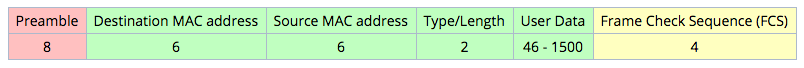
\includegraphics[width=0.9\textwidth]{ethernet.png}
	\caption{Ethernet Frame Structure}
	\label{fig:ethernet}
\end{figure}

\texttt{00 27 10 21 fa 48 00 13 \hspace{0.5cm} 10 e8 dd 52 08 06 00 01\\ 08 00 06 04 00 01 00 13 \hspace{0.5cm} 10 e8 dd 52 c0 a8 02 01\\ 00 00 00 00 00 00 c0 a8 \hspace{0.5cm} 02 67} \\ \\

\underline{Find}:
\begin{enumerate}
	\item Source MAC Address
	\item Destination MAC Address
	\item What protocol is inside the data payload?
	\item Please mention what the last 2 fields hold in the above frame.
\end{enumerate}

\underline{Answer}:

\begin{enumerate}
	\item Source MAC Address: \texttt{00:13:10:e8:dd:52}
	\item Destination MAC Address: \texttt{00:27:10:21:fa:48}
	\item Protocol: Address Resolution Protocol 
	\item The penultimate field is the targets MAC Address and the last field is the targets IP Address.
\end{enumerate}

\section{Cable Issue (5 Points)}

Let us consider we have two cables of 20 meters each. One of them is in a 100MBps network while the other is in a 10MBps network. If you had to transfer data through each of them, how much time it would take for the first bit to arrive in each setting? (For your calculation you can assume that the speed of light takes the same value as in the videos.) Please provide formulas and calculatoins along with your results.

\underline{Answer}:

Let $c$ be the speed of light, $l$ the length of the cable and $t$ the time it takes for the first bit to travel the length $l$. 
As the length of the cables are equal and the networks bandwidth doesn't change the propagation delay, the calculation for both networks are the same.  
Given the speed of light $c = 3 \cdot 10^8 \frac{m}{s}$ and the formula for the propagation delay $t = \frac{l}{c}$, the propagation delay is $t = \frac{20}{3 \cdot 10^8}s \approx 67ns$

\section{Basic Network Tools (10 Points)}

Listed below are some of the commands which you need to "google" to understand what they stand for:
\begin{enumerate}
	\item \emph{ipconfig / ifconfig}
	\item \emph{ping}
	\item \emph{traceroute}
	\item \emph{arp}
	\item \emph{dig}
\end{enumerate}

Consider a situation in which you need to check if \url{www.wikipedia.org} is reachable or not. Using the knowledge you gained above to \underline{find the following information}:
\begin{enumerate}
	\itemsep0em
	\item The \emph{\% packet loss} if at all it happened after sending 100 packets.
	\item \emph{Size} of the packet sent to \emph{Wikipedia} server
	\item \emph{IP address} of your machine and the \emph{Wikipedia} server
	\item \emph{Query Time} for DNS query of the above url.
	\item Number of \emph{Hops} in between your machine and the server
	\item MAC address of the device that is acting as your network gateway.
\end{enumerate}

Do this once in the university and once in your home/dormitory network. With your answers, you must paste the screen shots to validate your find.

\underline{Answer}:

\lstset{breaklines=true, frame=single}

\textbf{1.} The \% packet loss if at all it happened after sending 100 packets.

Home: 0\%

University: 0\%

\begin{lstlisting}[caption=ping home]
	ping -c 100 -i 0.2  www.wikipedia.de
	...
	100 packets transmitted, 100 received, 0% packet loss, time 19883ms
	rtt min/avg/max/mdev = 18.037/21.074/29.851/1.646 ms
\end{lstlisting}

\begin{lstlisting}[caption=ping university]
	100 packets transmitted, 100 received, 0% packet loss, time 19880ms
	rtt min/avg/max/mdev = 9.323/10.315/19.560/1.547 ms
\end{lstlisting}

\textbf{2.} Size of the packet sent to Wikipedia server.

Home: 64 bytes

University: 64 bytes

\begin{lstlisting}[caption=man ping]
	       -s packetsize
	                     Specifies the number of data bytes to be sent.  The default is 56, which translates into 64 ICMP data
			     bytes when combined with the 8 bytes of ICMP header data.
\end{lstlisting}

\textbf{3.} IP address of your machine and the Wikipedia server

Home: 192.168.2.115, 91.198.174.192

University: 141.26.186.205, 91.198.174.192

\begin{lstlisting}[caption=ifconfig home]
	ifconfig
	...
	bond0: flags=5187<UP,BROADCAST,RUNNING,MASTER,MULTICAST>  mtu 1500
	inet 192.168.2.115  netmask 255.255.255.0  broadcast 192.168.2.255
	inet6 fd21:22dd:f528:1:d6b5:5652:241e:f450  prefixlen 64  scopeid 0x0<global>
	inet6 fd21:22dd:f528:1:f2de:f1ff:fe03:c9c9  prefixlen 64  scopeid 0x0<global>
	inet6 2003:c5:5bd7:2653:d8fd:5b7d:730d:9337  prefixlen 64  scopeid 0x0<global>
	inet6 2003:c5:5bd7:2653:f2de:f1ff:fe03:c9c9  prefixlen 64  scopeid 0x0<global>
	inet6 fe80::f2de:f1ff:fe03:c9c9  prefixlen 64  scopeid 0x20<link>
	ether f0:de:f1:03:c9:c9  txqueuelen 1000  (Ethernet)
	RX packets 7563  bytes 6410345 (6.1 MiB)
	RX errors 0  dropped 0  overruns 0  frame 0
	TX packets 5621  bytes 1106251 (1.0 MiB)
	TX errors 0  dropped 0 overruns 0  carrier 0  collisions 0
\end{lstlisting}

\begin{lstlisting}[caption=arp www.wikipedia.org home]
	arp www.wikipedia.org
	...
	www.wikipedia.org (91.198.174.192) -- no entry	
\end{lstlisting}

\begin{lstlisting}[caption=ipconfig university]
	ifconfig
	...
	bond0: flags=5187<UP,BROADCAST,RUNNING,MASTER,MULTICAST>  mtu 1500
	inet 141.26.186.205  netmask 255.255.240.0  broadcast 141.26.191.255
	inet6 fe80::f2de:f1ff:fe03:c9c9  prefixlen 64  scopeid 0x20<link>
	ether f0:de:f1:03:c9:c9  txqueuelen 1000  (Ethernet)
	RX packets 16144  bytes 2051137 (1.9 MiB)
	RX errors 0  dropped 391  overruns 0  frame 0
	TX packets 148  bytes 18728 (18.2 KiB)
	TX errors 0  dropped 0 overruns 0  carrier 0  collisions 0
\end{lstlisting}

\begin{lstlisting}[caption=arp www.wikipedia.org university]
        arp www.wikipedia.org
        ...
        www.wikipedia.org (91.198.174.192) -- no entry  
\end{lstlisting}

\textbf{4.} Query Time for DNS query of the above url.

Home: 3msec

University: 82msec

\begin{lstlisting}[caption=dig home]
	dig www.wikipedia.org
	...
	; <<>> DiG 9.11.0 <<>> www.wikipedia.org
	;; global options: +cmd
	;; Got answer:
	;; ->>HEADER<<- opcode: QUERY, status: NOERROR, id: 7395
	;; flags: qr rd ra ad; QUERY: 1, ANSWER: 1, AUTHORITY: 0, ADDITIONAL: 0

	;; QUESTION SECTION:
	;wikipedia.org.			IN	A

	;; ANSWER SECTION:
	www.wikipedia.org.		38	IN	A	91.198.174.192

	;; Query time: 3 msec
	;; SERVER: 192.168.2.1#53(192.168.2.1)
	;; WHEN: Wed Nov 02 06:22:14 UTC 2016
	;; MSG SIZE  rcvd: 47
\end{lstlisting}

\begin{lstlisting}
	dig www.wikipedia.org
	...
	; <<>> DiG 9.11.0 <<>> www.wikipedia.org
	;; global options: +cmd
	;; Got answer:
	;; ->>HEADER<<- opcode: QUERY, status: NOERROR, id: 478
	;; flags: qr rd ra; QUERY: 1, ANSWER: 1, AUTHORITY: 6, ADDITIONAL: 13

	;; OPT PSEUDOSECTION:
	; EDNS: version: 0, flags:; udp: 4096
	;; QUESTION SECTION:
	;www.wikipedia.org.		IN	A

	;; ANSWER SECTION:
	www.wikipedia.org.	456	IN	A	91.198.174.192

	;; AUTHORITY SECTION:
	org.			165879	IN	NS	c0.org.afilias-nst.info.
	org.			165879	IN	NS	d0.org.afilias-nst.org.
	org.			165879	IN	NS	a0.org.afilias-nst.info.
	org.			165879	IN	NS	a2.org.afilias-nst.info.
	org.			165879	IN	NS	b2.org.afilias-nst.org.
	org.			165879	IN	NS	b0.org.afilias-nst.org.

	;; ADDITIONAL SECTION:
	a0.org.afilias-nst.info. 165879	IN	A	199.19.56.1
	a0.org.afilias-nst.info. 165879	IN	AAAA	2001:500:e::1
	a2.org.afilias-nst.info. 165879	IN	A	199.249.112.1
	a2.org.afilias-nst.info. 165879	IN	AAAA	2001:500:40::1
	b0.org.afilias-nst.org.	165879	IN	A	199.19.54.1
	b0.org.afilias-nst.org.	165879	IN	AAAA	2001:500:c::1
	b2.org.afilias-nst.org.	165879	IN	A	199.249.120.1
	b2.org.afilias-nst.org.	165879	IN	AAAA	2001:500:48::1
	c0.org.afilias-nst.info. 165879	IN	A	199.19.53.1
	c0.org.afilias-nst.info. 165879	IN	AAAA	2001:500:b::1
	d0.org.afilias-nst.org.	165879	IN	A	199.19.57.1
	d0.org.afilias-nst.org.	165879	IN	AAAA	2001:500:f::1

	;; Query time: 81 msec
	;; SERVER: 141.26.64.60#53(141.26.64.60)
	;; WHEN: Wed Nov 02 07:51:43 UTC 2016
	;; MSG SIZE  rcvd: 464
\end{lstlisting}

\textbf{5.} Number of Hops in between your machine and the server

Home: didn't complete after 100+ hops

University: 11

\begin{lstlisting}[caption=traceroute university]
	traceroute -I www.wikipedia.org
	...
	traceroute to www.wikipedia.org (91.198.174.192), 30 hops max, 60 byte packets
	1  wlanrouter.uni-koblenz.de (141.26.176.1)  3.303 ms  6.096 ms  6.104 ms
	2  g-uni-ko-1.rlp-net.net (217.198.241.129)  6.123 ms  6.124 ms  8.683 ms
	3  g-hbf-ko-1.rlp-net.net (217.198.240.69)  6.102 ms  8.684 ms  8.684 ms
	4  g-hbf-mz-2.rlp-net.net (217.198.240.21)  8.684 ms  8.684 ms  11.187 ms
	5  g-interxion-1.rlp-net.net (217.198.240.13)  11.206 ms  14.308 ms  14.319 ms
	6  r1fra3.core.init7.net (80.81.192.67)  14.327 ms  5.593 ms  4.234 ms
	7  r1ams1.core.init7.net (77.109.128.154)  16.680 ms  16.691 ms  16.697 ms
	8  r1ams2.core.init7.net (77.109.128.146)  18.935 ms  18.934 ms  19.091 ms
	9  gw-wikimedia.init7.net (77.109.134.114)  18.920 ms  18.915 ms  18.909 ms
	10  ae1-403.cr2-esams.wikimedia.org (91.198.174.254)  18.904 ms  18.914 ms  18.888 ms
	11  text-lb.esams.wikimedia.org (91.198.174.192)  18.898 ms  21.779 ms  21.767 ms
\end{lstlisting}

\textbf{6.} MAC address of the device that is acting as your network gateway.

Home: d4:21:22:dd:f5:28

University: 14:18:77:45:b1:bd 

\begin{lstlisting}[caption=arp home]
	arp -n
	...
	Address                  HWtype  HWaddress           Flags Mask            Iface
	192.168.2.1              ether   d4:21:22:dd:f5:28   C                     bond0
\end{lstlisting}

\begin{lstlisting}[caption=arp university]
	arp -n
	...
	Address                  HWtype  HWaddress           Flags Mask            Iface
	141.26.176.1             ether   14:18:77:45:b1:bd   C                     bond
\end{lstlisting}


\section{Simple Python Programming}

Write a simple \underline{python program that does the following}:
\begin{enumerate}
	\item Generate a random number sequence of 10 values between 0 to 90.
	\item Perform \texttt{sine} and \texttt{cosine} operation on numbers generated.
	\item Store the values in two different arrays named SIN \& COSIN respectively.
	\item Plot the values of SIN \& COSIN in two different colors.
	\item The plot should have labeled axes and legend.
\end{enumerate}

\underline{Answer}:

\lstset{language=python, breaklines=true, frame=single}
\lstinputlisting{tango_assignment1_4.py}

\end{document}
